\chapter{CloudTrail}\label{ch:cloudtrail}

The use of CloudTrail will allow for logging across the project.
This will give the group control over storage, analysis and any remediation actions.
Visibility of AWS account activity is a recommended AWS security best practice~\parencite{amazon2022cloudtrail}.

CloudTrail will be enabled for any changes which occur within the project's S3 bucket and RDS instances.
The CloudTrail is first given the name of~\mintinline{zsh}|Group4-CloudTrail|.
A location for the logs that CloudTrail outputs is required, so the S3 bucket created in
Chapter~\ref{ch:simple-storage-service} is selected as the storage location.
The "Log file SSE-KMS encryption" option is Enabled, which encrypts the log files that are generated, heightening
security.
A KMS is required to encrypt this data, and a new one is created and named~\mintinline{zsh}|Group4-kms|.
These options can be seen in Figure~\ref{fig:cloudwatch-general-1}.

\begin{figure}[!htbp]
    \centering
    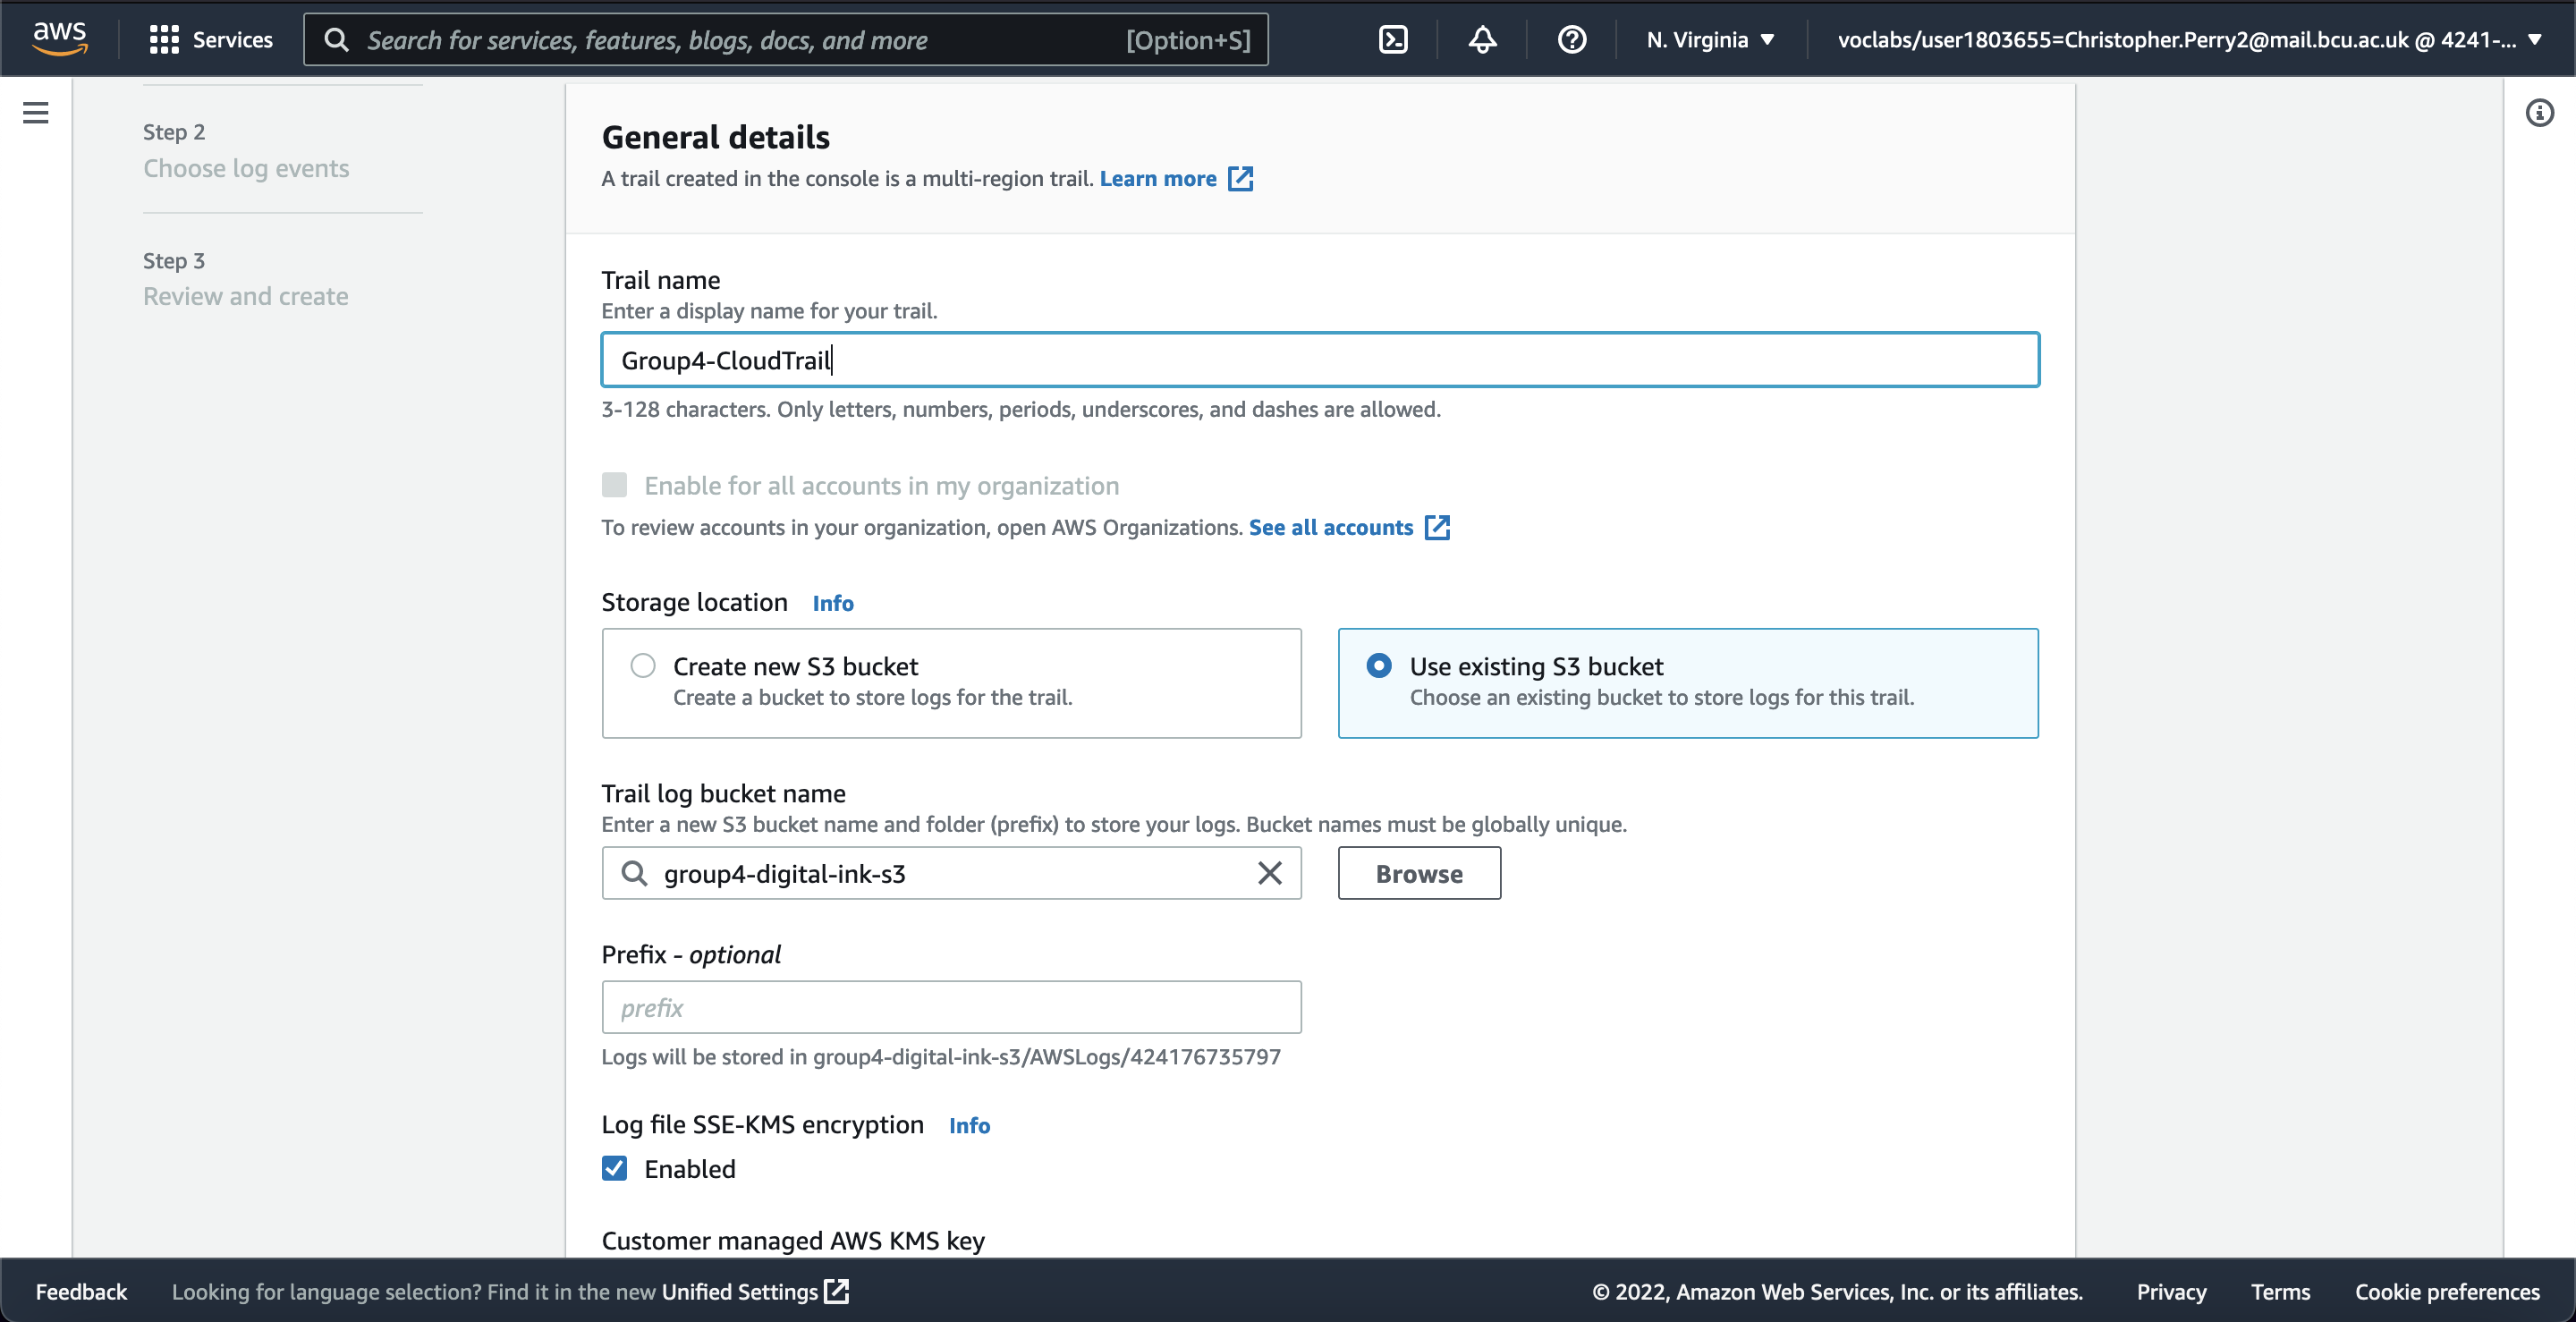
\includegraphics[width=\textwidth]{resources/cloudtrail/cloudtrail-general-1}
    \caption{Initial CloudTrail set up.}
    \label{fig:cloudwatch-general-1}
\end{figure}

The "Log file validation" option is selected, which ensures that any changes which have been to made to the log file
that are not from CloudTrail directly are notified to the group.
These aforementioned notifications have been set up through the creation of new SNS topic
called~\mintinline{zsh}|Group4-cloudtrail-sns|.
These options can be seen in Figure~\ref{fig:cloudwatch-general-2}.

\begin{figure}[!htbp]
    \centering
    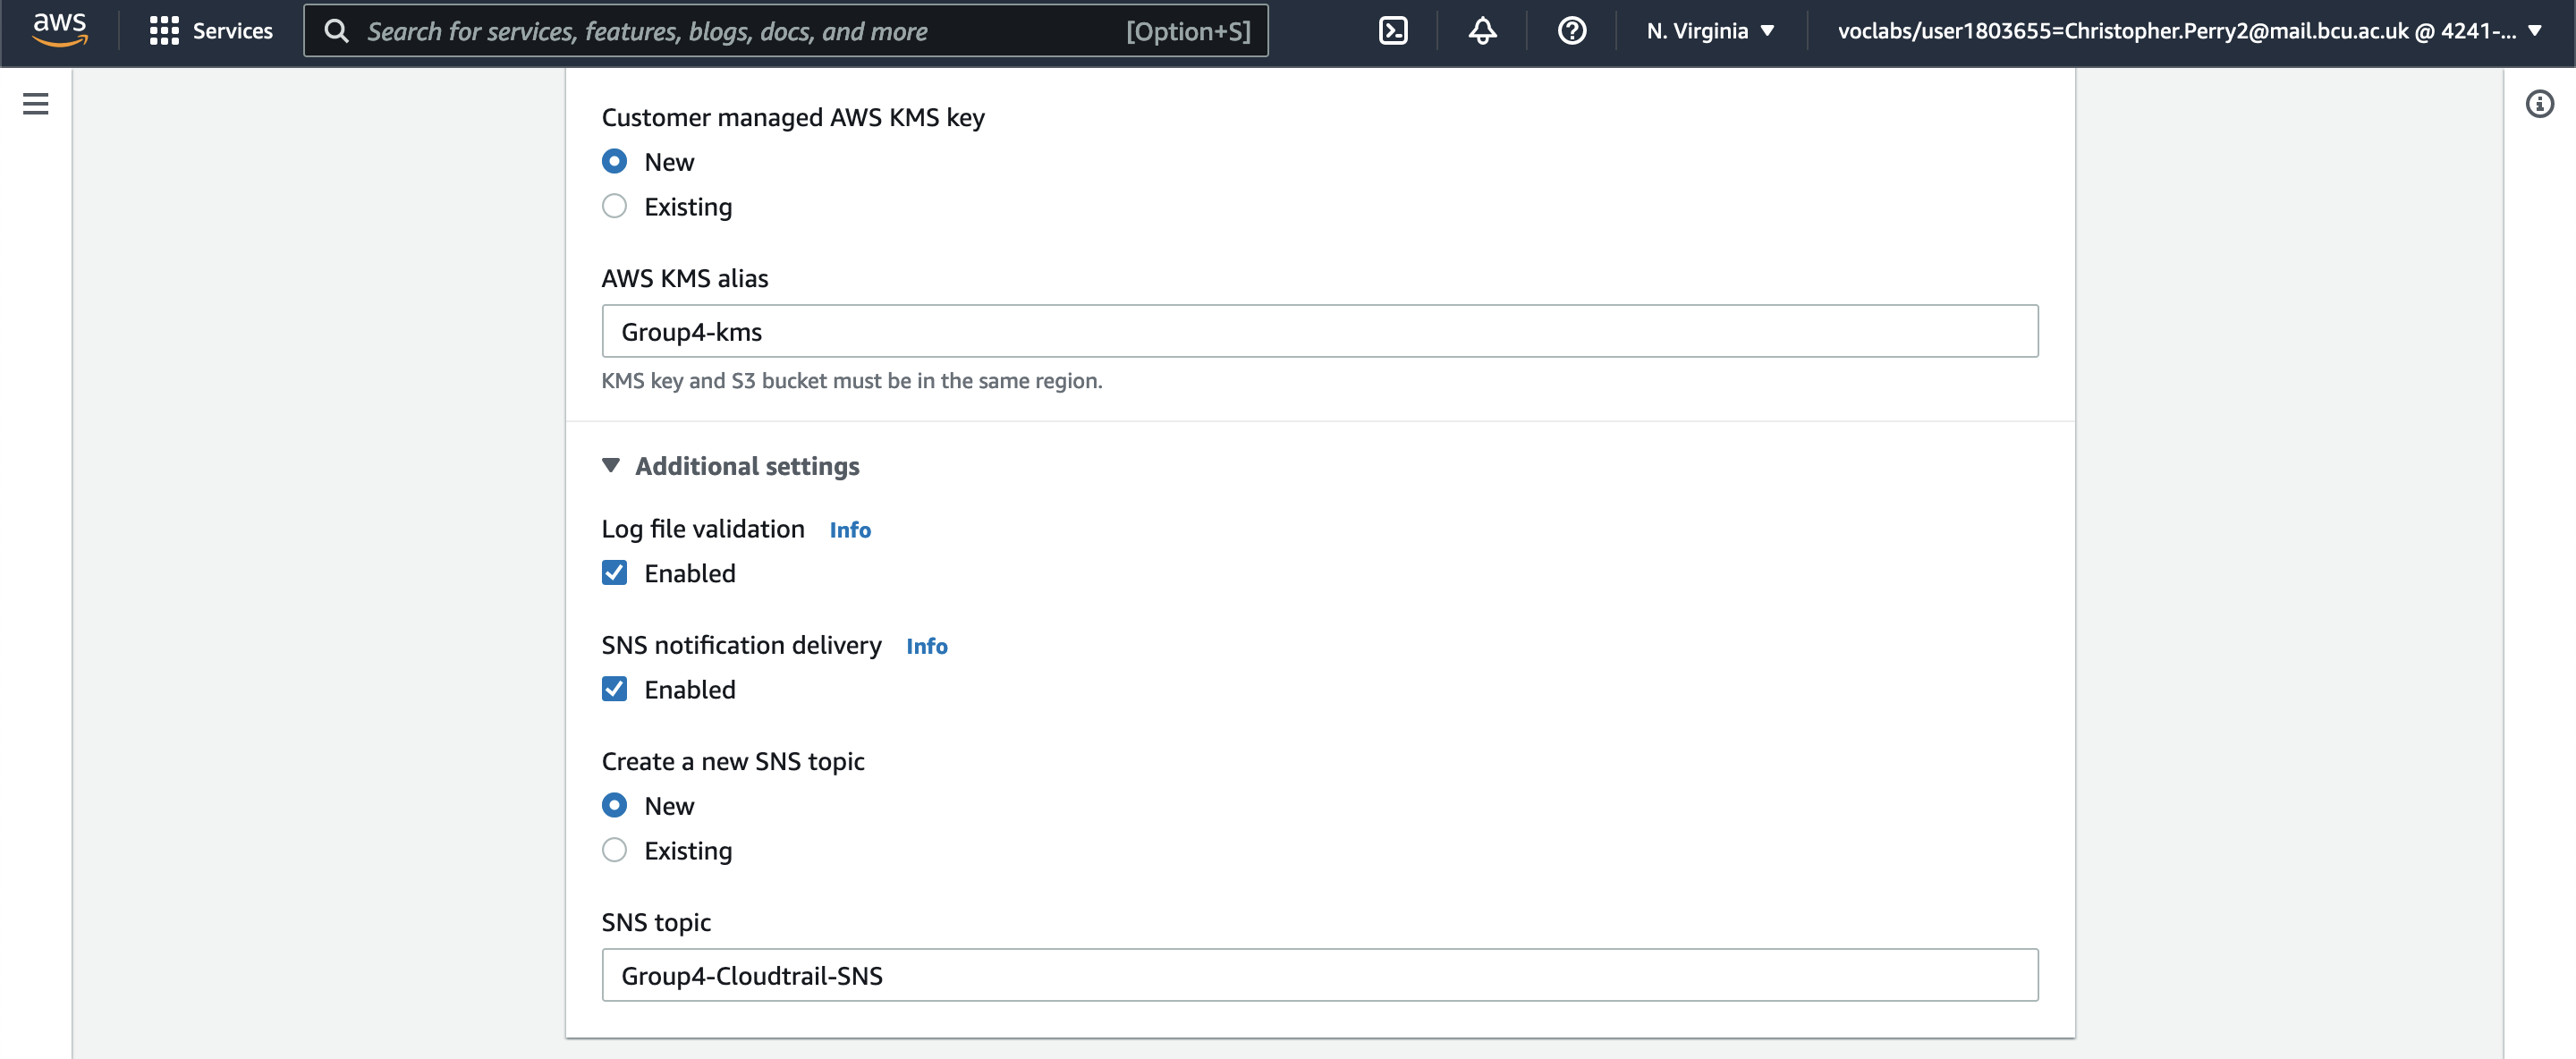
\includegraphics[width=\textwidth]{resources/cloudtrail/cloudtrail-general-2}
    \caption{Initial CloudTrail set up.}
    \label{fig:cloudwatch-general-2}
\end{figure}

\clearpage

Now that the CloudTrail initial setup is complete, the selection of the specific events which will be monitored can be
configured.
"Management Events" is firstly selected - this will allow for any read or write events which have been applied on
the S3 and RDS services to be logged.
In addition to this, "Insights Events" is also enabled, which will allow for any unusual activity on these services to
also be logged through the use of the API Call Rate and Error Rate - If they are high, this will be logged via CloudTrail.
which is of a security benefit to the project.

These settings can be seen configured in Figures~\ref{fig:cloudwatch-events-1} and~\ref{fig:cloudwatch-events-2}.

\begin{figure}[!htbp]
    \centering
    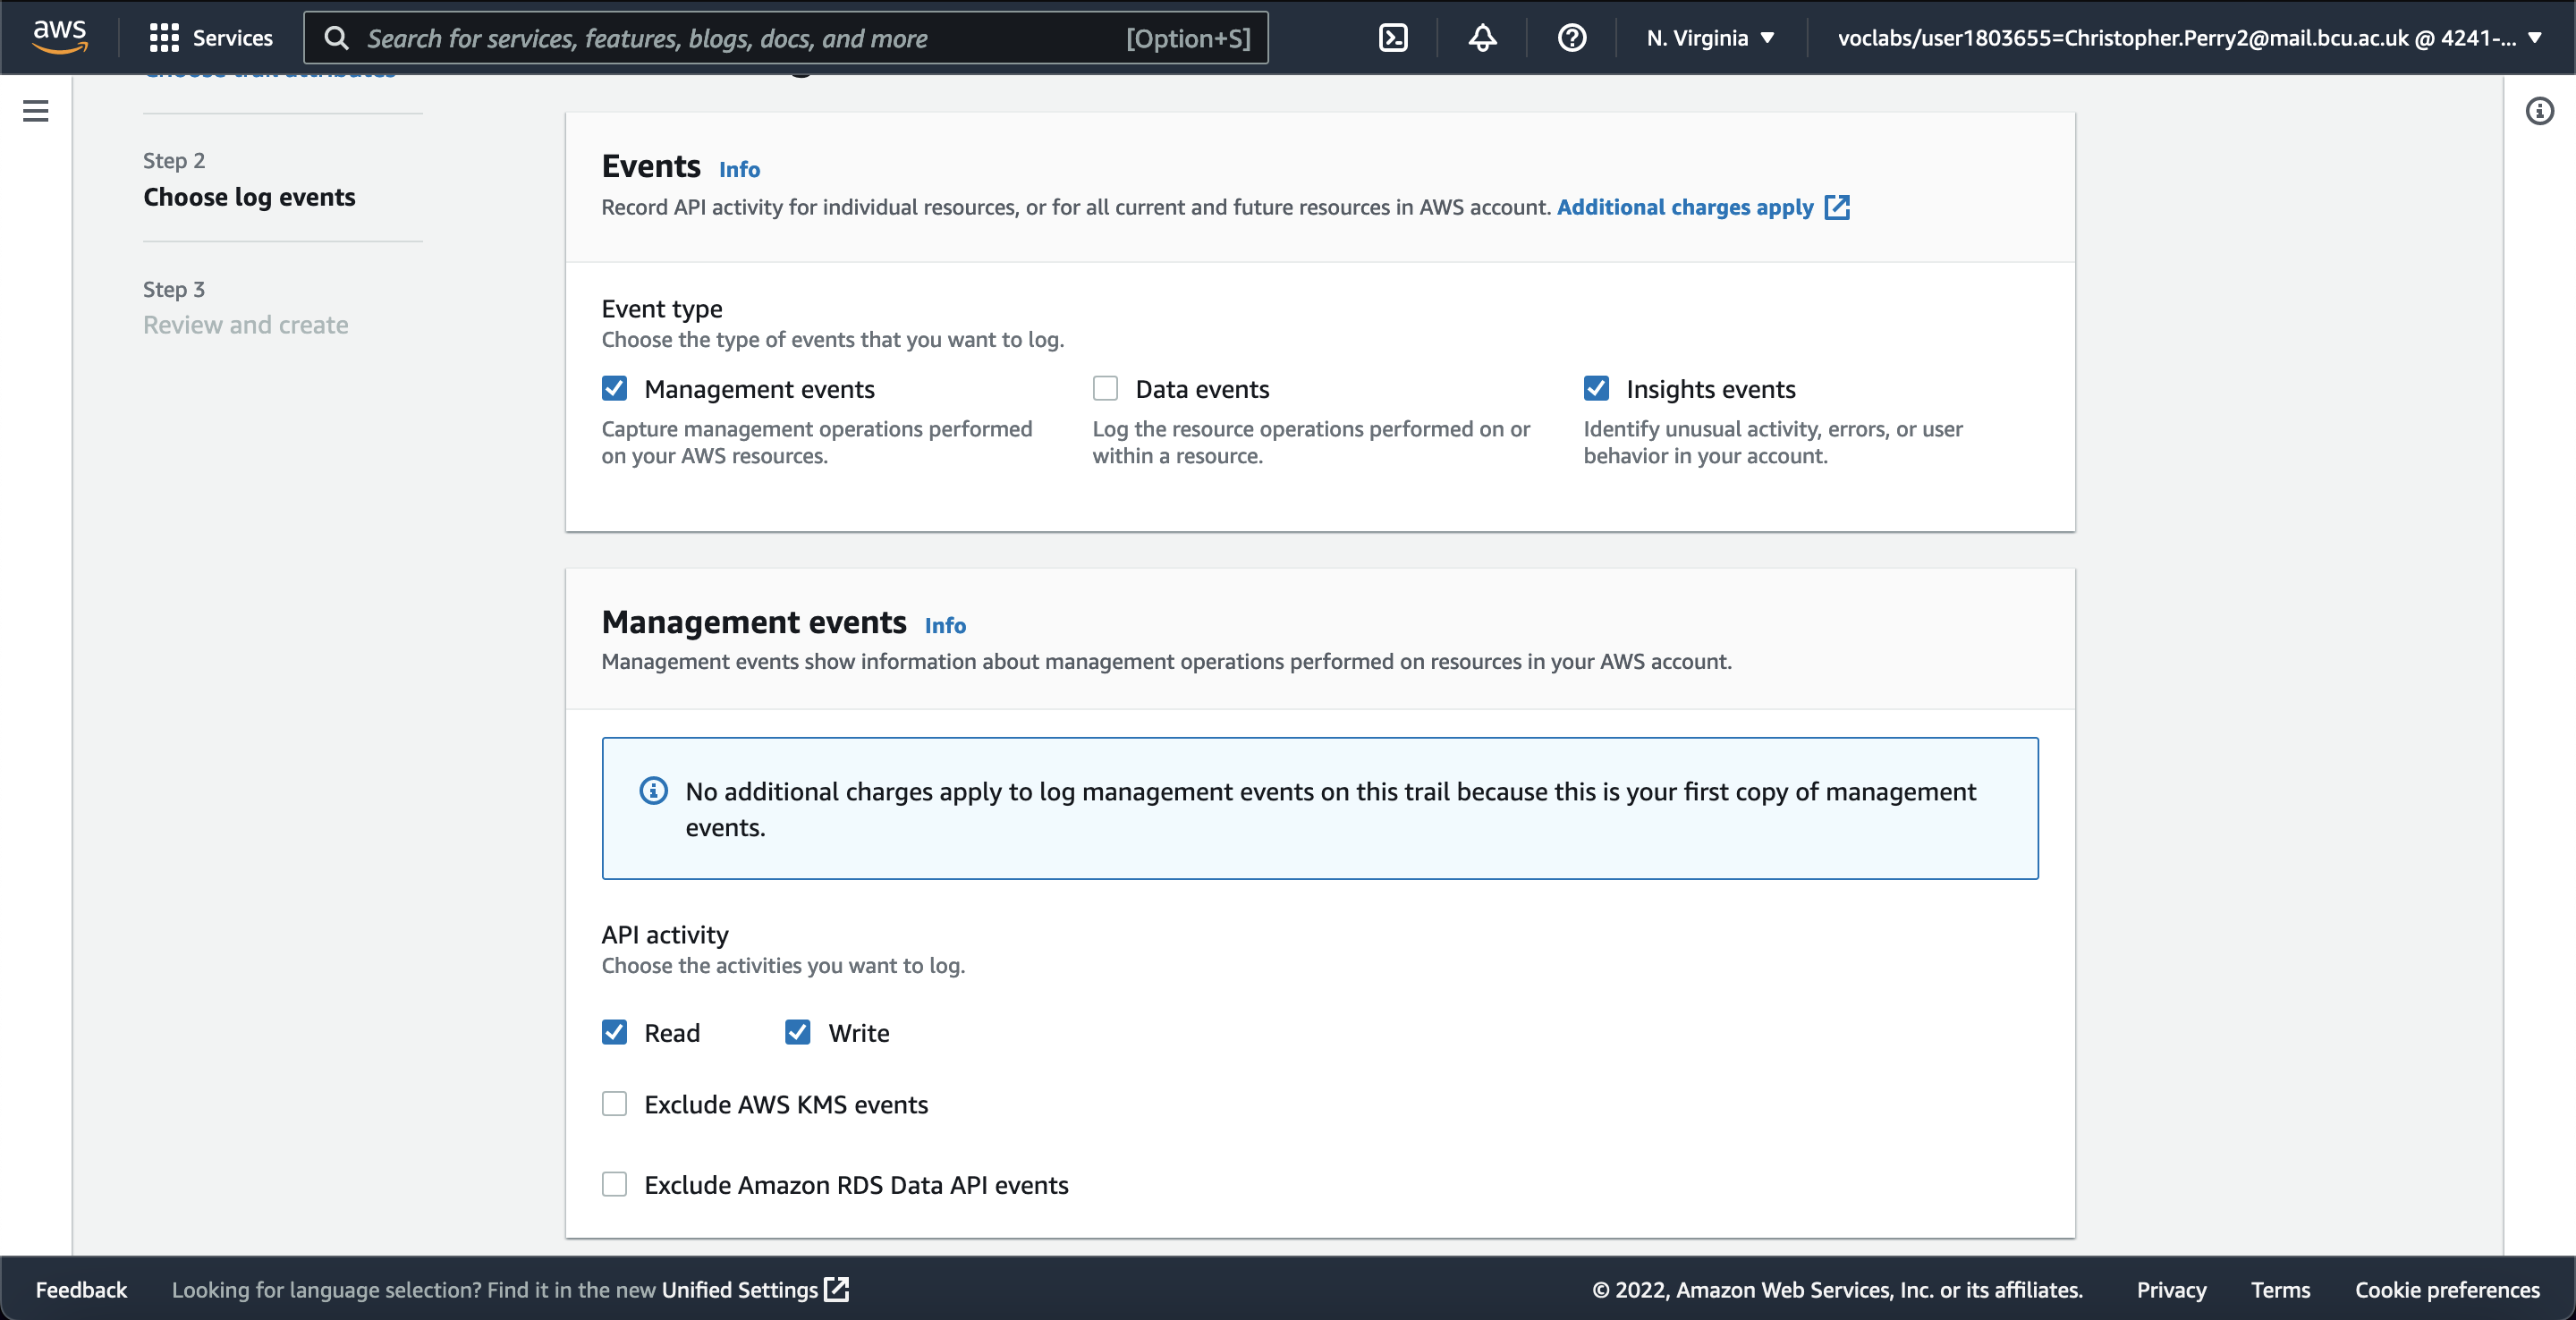
\includegraphics[width=\textwidth]{resources/cloudtrail/cloudtrail-events-1}
    \caption{Configuring CloudTrail events.}
    \label{fig:cloudwatch-events-1}
\end{figure}


\begin{figure}[!htbp]
    \centering
    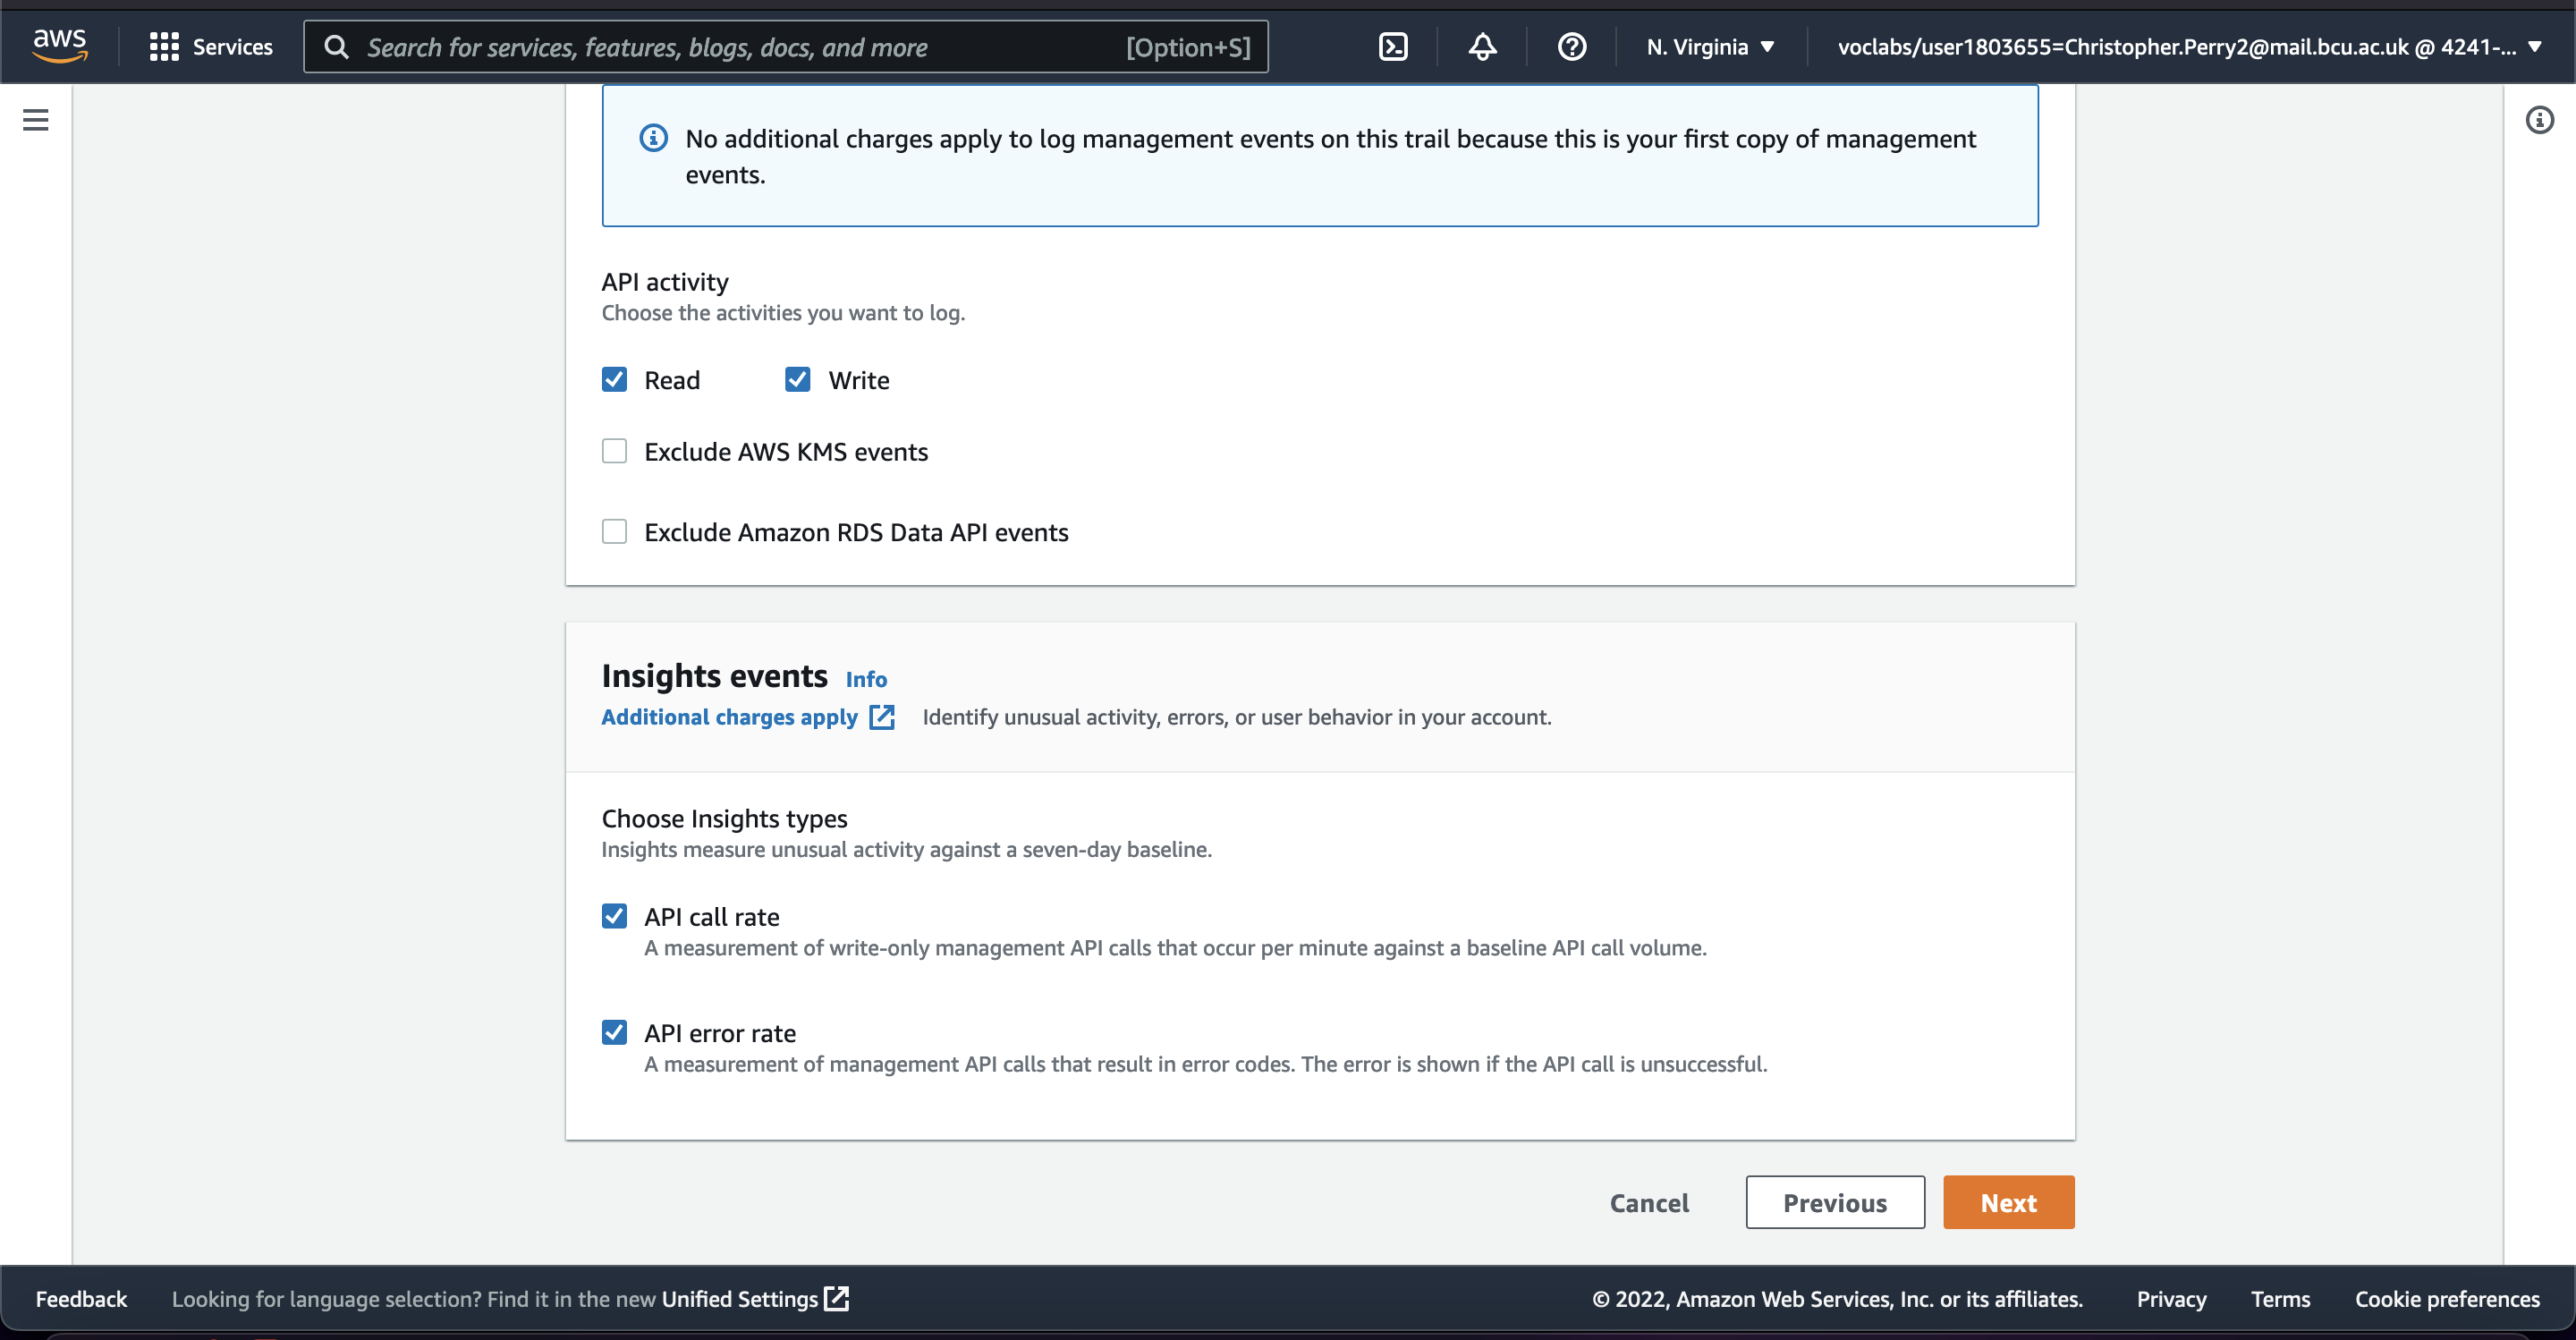
\includegraphics[width=\textwidth]{resources/cloudtrail/cloudtrail-events-2}
    \caption{Configuring CloudTrail events.}
    \label{fig:cloudwatch-events-2}
\end{figure}

The CloudTrail has now been added and is now monitoring for any activity.
This can be seen in Figure~\ref{fig:cloudtrail-added}.

\begin{figure}[!htbp]
    \centering
    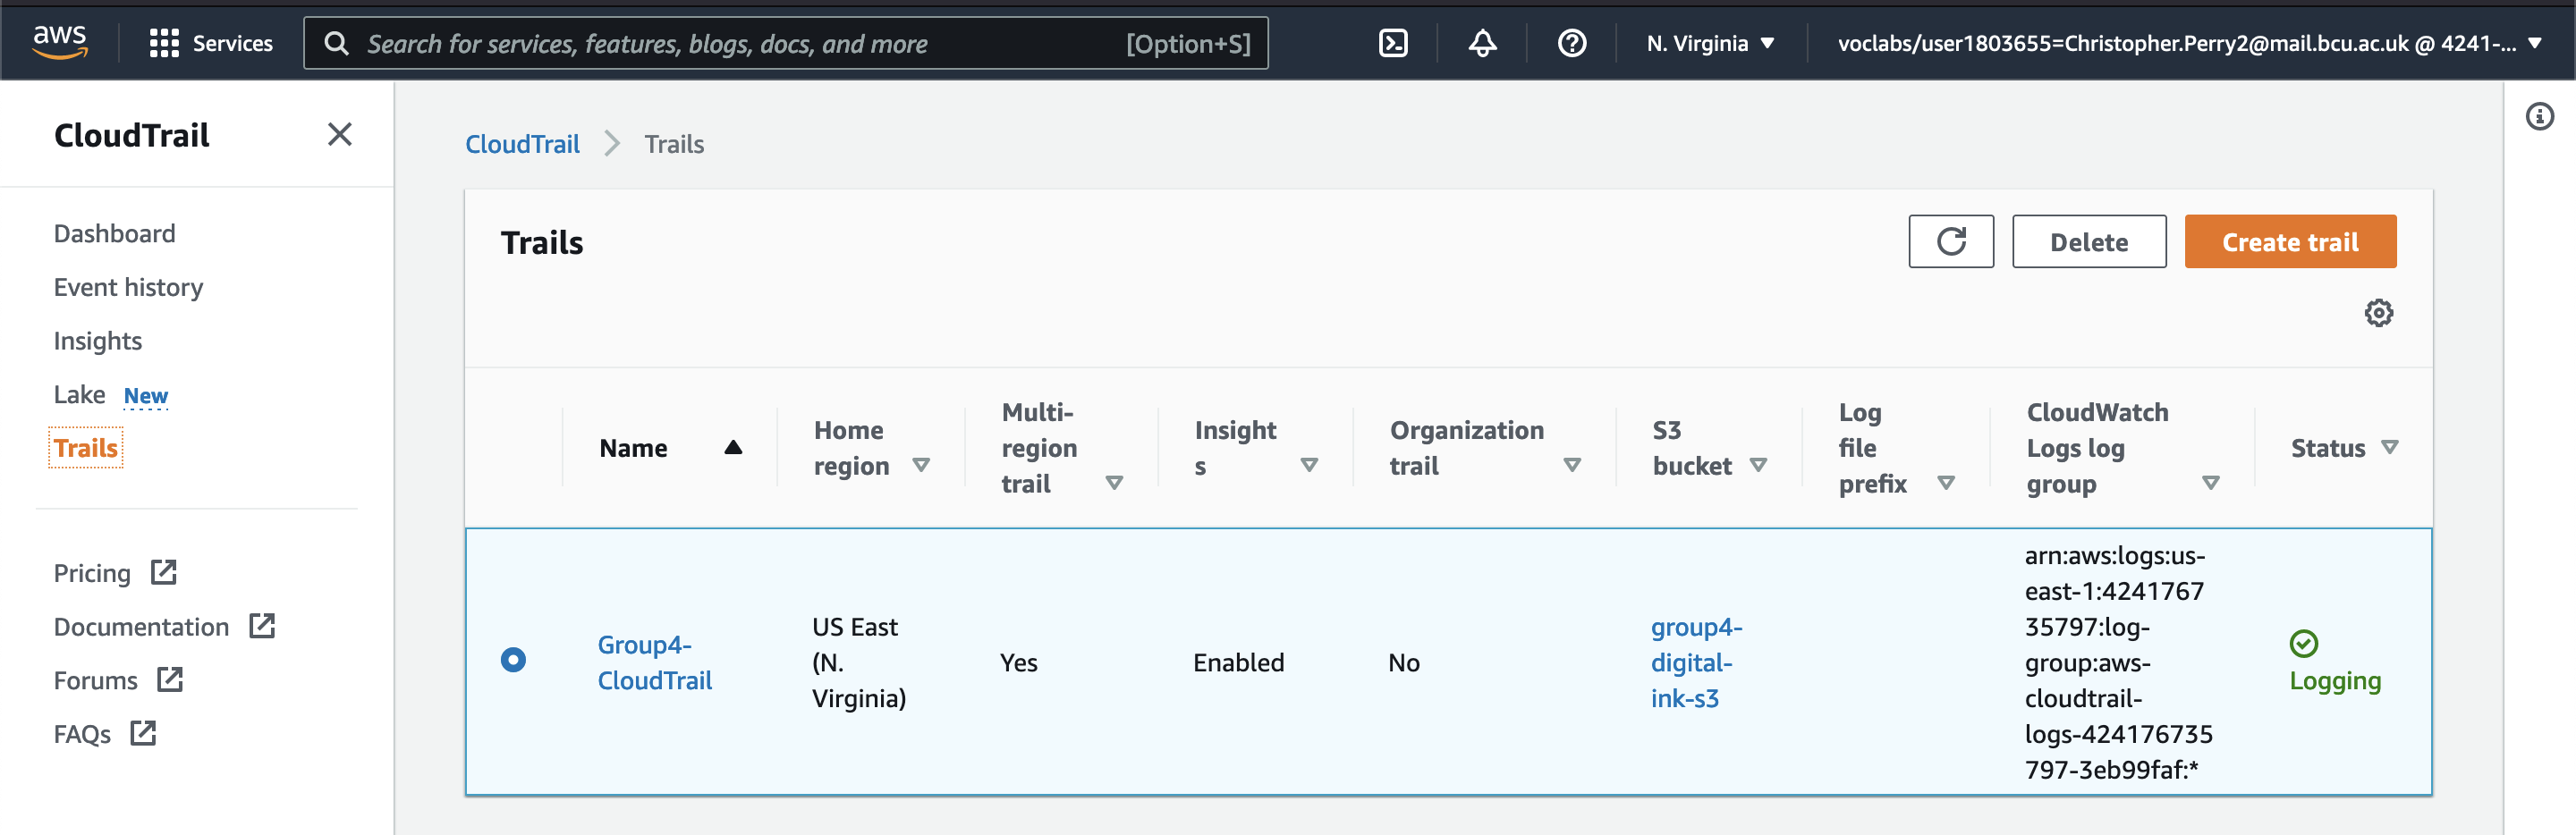
\includegraphics[width=\textwidth]{resources/cloudtrail/cloudtrail-added}
    \caption{Added CloudTrail instance.}
    \label{fig:cloudtrail-added}
\end{figure}



